\documentclass[10pt,ignorenonframetext,]{beamer}
\setbeamertemplate{caption}[numbered]
\setbeamertemplate{caption label separator}{: }
\setbeamercolor{caption name}{fg=normal text.fg}
\beamertemplatenavigationsymbolsempty
\usepackage{lmodern}
\usepackage{amssymb,amsmath}
\usepackage{ifxetex,ifluatex}
\usepackage{fixltx2e} % provides \textsubscript
\ifnum 0\ifxetex 1\fi\ifluatex 1\fi=0 % if pdftex
\usepackage[T1]{fontenc}
\usepackage[utf8]{inputenc}
\else % if luatex or xelatex
\ifxetex
\usepackage{mathspec}
\else
\usepackage{fontspec}
\fi
\defaultfontfeatures{Ligatures=TeX,Scale=MatchLowercase}
\fi
% use upquote if available, for straight quotes in verbatim environments
\IfFileExists{upquote.sty}{\usepackage{upquote}}{}
% use microtype if available
\IfFileExists{microtype.sty}{%
\usepackage{microtype}
\UseMicrotypeSet[protrusion]{basicmath} % disable protrusion for tt fonts
}{}
\newif\ifbibliography
\usepackage{color}
\usepackage{fancyvrb}
\newcommand{\VerbBar}{|}
\newcommand{\VERB}{\Verb[commandchars=\\\{\}]}
\DefineVerbatimEnvironment{Highlighting}{Verbatim}{commandchars=\\\{\}}
% Add ',fontsize=\small' for more characters per line
\usepackage{framed}
\definecolor{shadecolor}{RGB}{248,248,248}
\newenvironment{Shaded}{\begin{snugshade}}{\end{snugshade}}
\newcommand{\KeywordTok}[1]{\textcolor[rgb]{0.13,0.29,0.53}{\textbf{{#1}}}}
\newcommand{\DataTypeTok}[1]{\textcolor[rgb]{0.13,0.29,0.53}{{#1}}}
\newcommand{\DecValTok}[1]{\textcolor[rgb]{0.00,0.00,0.81}{{#1}}}
\newcommand{\BaseNTok}[1]{\textcolor[rgb]{0.00,0.00,0.81}{{#1}}}
\newcommand{\FloatTok}[1]{\textcolor[rgb]{0.00,0.00,0.81}{{#1}}}
\newcommand{\ConstantTok}[1]{\textcolor[rgb]{0.00,0.00,0.00}{{#1}}}
\newcommand{\CharTok}[1]{\textcolor[rgb]{0.31,0.60,0.02}{{#1}}}
\newcommand{\SpecialCharTok}[1]{\textcolor[rgb]{0.00,0.00,0.00}{{#1}}}
\newcommand{\StringTok}[1]{\textcolor[rgb]{0.31,0.60,0.02}{{#1}}}
\newcommand{\VerbatimStringTok}[1]{\textcolor[rgb]{0.31,0.60,0.02}{{#1}}}
\newcommand{\SpecialStringTok}[1]{\textcolor[rgb]{0.31,0.60,0.02}{{#1}}}
\newcommand{\ImportTok}[1]{{#1}}
\newcommand{\CommentTok}[1]{\textcolor[rgb]{0.56,0.35,0.01}{\textit{{#1}}}}
\newcommand{\DocumentationTok}[1]{\textcolor[rgb]{0.56,0.35,0.01}{\textbf{\textit{{#1}}}}}
\newcommand{\AnnotationTok}[1]{\textcolor[rgb]{0.56,0.35,0.01}{\textbf{\textit{{#1}}}}}
\newcommand{\CommentVarTok}[1]{\textcolor[rgb]{0.56,0.35,0.01}{\textbf{\textit{{#1}}}}}
\newcommand{\OtherTok}[1]{\textcolor[rgb]{0.56,0.35,0.01}{{#1}}}
\newcommand{\FunctionTok}[1]{\textcolor[rgb]{0.00,0.00,0.00}{{#1}}}
\newcommand{\VariableTok}[1]{\textcolor[rgb]{0.00,0.00,0.00}{{#1}}}
\newcommand{\ControlFlowTok}[1]{\textcolor[rgb]{0.13,0.29,0.53}{\textbf{{#1}}}}
\newcommand{\OperatorTok}[1]{\textcolor[rgb]{0.81,0.36,0.00}{\textbf{{#1}}}}
\newcommand{\BuiltInTok}[1]{{#1}}
\newcommand{\ExtensionTok}[1]{{#1}}
\newcommand{\PreprocessorTok}[1]{\textcolor[rgb]{0.56,0.35,0.01}{\textit{{#1}}}}
\newcommand{\AttributeTok}[1]{\textcolor[rgb]{0.77,0.63,0.00}{{#1}}}
\newcommand{\RegionMarkerTok}[1]{{#1}}
\newcommand{\InformationTok}[1]{\textcolor[rgb]{0.56,0.35,0.01}{\textbf{\textit{{#1}}}}}
\newcommand{\WarningTok}[1]{\textcolor[rgb]{0.56,0.35,0.01}{\textbf{\textit{{#1}}}}}
\newcommand{\AlertTok}[1]{\textcolor[rgb]{0.94,0.16,0.16}{{#1}}}
\newcommand{\ErrorTok}[1]{\textcolor[rgb]{0.64,0.00,0.00}{\textbf{{#1}}}}
\newcommand{\NormalTok}[1]{{#1}}
\usepackage{longtable,booktabs}
\usepackage{caption}
% These lines are needed to make table captions work with longtable:
\makeatletter
\def\fnum@table{\tablename~\thetable}
\makeatother
\usepackage{graphicx,grffile}
\makeatletter
\def\maxwidth{\ifdim\Gin@nat@width>\linewidth\linewidth\else\Gin@nat@width\fi}
\def\maxheight{\ifdim\Gin@nat@height>\textheight0.8\textheight\else\Gin@nat@height\fi}
\makeatother
% Scale images if necessary, so that they will not overflow the page
% margins by default, and it is still possible to overwrite the defaults
% using explicit options in \includegraphics[width, height, ...]{}
\setkeys{Gin}{width=\maxwidth,height=\maxheight,keepaspectratio}

% Prevent slide breaks in the middle of a paragraph:
\widowpenalties 1 10000
\raggedbottom

\AtBeginPart{
\let\insertpartnumber\relax
\let\partname\relax
\frame{\partpage}
}
\AtBeginSection{
\ifbibliography
\else
\let\insertsectionnumber\relax
\let\sectionname\relax
\frame{\sectionpage}
\fi
}
\AtBeginSubsection{
\let\insertsubsectionnumber\relax
\let\subsectionname\relax
\frame{\subsectionpage}
}

\setlength{\parindent}{0pt}
\setlength{\parskip}{6pt plus 2pt minus 1pt}
\setlength{\emergencystretch}{3em}  % prevent overfull lines
\providecommand{\tightlist}{%
\setlength{\itemsep}{0pt}\setlength{\parskip}{0pt}}
\setcounter{secnumdepth}{0}

\title{STA305/1004 - Class 3}
\date{January 16, 2017}

\begin{document}
\frame{\titlepage}

\begin{frame}{Today's Class}

\begin{itemize}
\tightlist
\item
  The concepts of: Randomization, Blocking, Replication
\item
  Summaries of sample populations
\item
  Hypothesis testing via randomization
\end{itemize}

\end{frame}

\begin{frame}{Randomized Experiments and Observational Studies}

\begin{itemize}
\tightlist
\item
  A technical definition of an observational study is given by Imbens
  and Rubin (2015)
\item
  The process that determines which experimental units receive which
  treatments is called the assignment mechanisim.
\item
  When the assignment mechanism is unknown then the design is called an
  observational study.
\end{itemize}

\end{frame}

\begin{frame}{Randomized Experiments and Observational Studies}

In randomized experiments (pg. 20, Imbens and Rubin, 2015): ``\ldots{}
the assignment mechanism is under the control of the experimenter, and
the probability of any assignment of treatments across the units in the
experiment is entirely knowable before the experiment begins.''

\end{frame}

\begin{frame}{Treatment Assignment}

Suppose, for example, that we have two breast cancer patients and we
want to randomly assign these two patients to two treatments (A and B).
Then how many ways can this be done?

\begin{enumerate}
\def\labelenumi{\arabic{enumi}.}
\tightlist
\item
  patient 1 receives A and patient 2 receives A
\item
  patient 1 receives A and patient 2 receives B
\item
  patient 1 receives B and patient 2 receives A
\item
  patient 1 receives B and patient 2 receives B
\end{enumerate}

\begin{itemize}
\tightlist
\item
  There are 4 possible treatment assignments.
\item
  The probability of a treatment assignment is 1/4,
\item
  The probability that an individual patient receives treatment A (or B)
  is 1/2.\\
\item
  In general, if there are \(N\) experimental units then there are
  \(2^N\) possible treatment assignments (provided there are two
  treatments).
\end{itemize}

\end{frame}

\begin{frame}{Treatment Assignment}

A treatment assignment vector records the treatmemnt that each
experimental unit is assigned to receive. If \(N=2\) then the possible
treatment assignment vectors are:

\[\begin{pmatrix} 
  1 \\
  0
 \end{pmatrix}, \begin{pmatrix}
 0 \\
  1
 \end{pmatrix},\begin{pmatrix}
 1 \\
  1
 \end{pmatrix},\begin{pmatrix}
 0 \\
  0
 \end{pmatrix},\]

where 1= treatment A, and 0=treatment B.

\end{frame}

\begin{frame}{Treatment Assignment}

\begin{itemize}
\tightlist
\item
  It wouldn't be a very imformative expriment if both patients received
  A or both received B.\\
\item
  Therefore, it makes sense to rule out this scenario.\\
\item
  We want to assign treatments to patients such that one patient
  receives A and the other receives B.
\item
  The possibile treatment assignments are:
\end{itemize}

\begin{enumerate}
\def\labelenumi{\arabic{enumi}.}
\item
  patient 1 receives A and patient 2 receives B or (in vector notation)
  \(\begin{pmatrix}  1 \\  0  \end{pmatrix}.\)
\item
  patient 1 receives B and patient 2 receives A or (in vector notation)
  \(\begin{pmatrix}  0 \\  1\end{pmatrix}.\)
\end{enumerate}

\begin{itemize}
\tightlist
\item
  In this case the probability of a treatment assignment is 1/2, and the
  probability that an individual patient receives treatment A (or B) is
  still 1/2.
\end{itemize}

\end{frame}

\begin{frame}{Randomized Experiments and Observational Studies}

Randomized experiments are currently viewed as the most credible basis
for determining cause and effect relationships. Health Canada, the U.S.
Food and Drug Administration, European Medicines Agency, and other
regulatory agencies all rely on randomized experiments in their approval
processes for pharmaceutical treatments.

\end{frame}

\begin{frame}{Randomization}

\begin{itemize}
\tightlist
\item
  The primary objective in the design of experiments is the avoidance of
  bias or systematic error (Cox and Reid, 2005).
\item
  One way to avoid bias is to use randomization.
\end{itemize}

\end{frame}

\begin{frame}{Randomization}

\begin{itemize}
\tightlist
\item
  Applied to the allocation of experimental units to treatments.
\item
  Provides protection to experimenter against variables unknown to
  experimenter but may impact the response.
\item
  Reduces influence of subjective judgement in treatment allocation.
\end{itemize}

\end{frame}

\begin{frame}{Randomization}

\begin{itemize}
\tightlist
\item
  National supported work demonstration program (NSW) included a
  randomized experiment to evaluate the effect of on the job training on
  unemployment. (Ref: Rosenbaum, pg. 22- 28)
\item
  Treatment: work experience in form of subsidized employment then
  individuals transitioned to unsubsidized employment.
\item
  Control: standard social programs
\end{itemize}

\end{frame}

\begin{frame}{Randomization}

\begin{itemize}
\tightlist
\item
  The response was earnings (\$) in 1978.
\item
  Later in course we will compare this with observational studies.
\item
  So participants were matched on pre-treatment covariates.
\item
  Results in 185 treated men matched to 185 treated controls.
\end{itemize}

\end{frame}

\begin{frame}{Randomization}

\begin{longtable}[]{@{}lll@{}}
\toprule
Covariate & Group & Earnings (\$)\tabularnewline
\midrule
\endhead
Age (Mean) & Treated & 25.82\tabularnewline
& Control & 25.70\tabularnewline
& &\tabularnewline
Years of education (Mean) & Treated & 10.35\tabularnewline
& Control & 10.19\tabularnewline
& &\tabularnewline
Black (\%) & Treated & 84\%\tabularnewline
& Control & 85\%\tabularnewline
& &\tabularnewline
Married (\%) & Treated & 19\%\tabularnewline
& Control & 20\%\tabularnewline
& &\tabularnewline
Earnings in 1974 \$ (Mean) & Treated & 2096\tabularnewline
& Control & 2009\tabularnewline
\bottomrule
\end{longtable}

\end{frame}

\begin{frame}{Blocking}

\begin{itemize}
\item
  To block an experiment is to divide the observations into groups
  called blocks so that observations in a block are collected under
  relatively similar conditions.
\item
  Suppose that the yield of a manufacturing process for penicillin
  varies a lot depending on how much of a certain raw material is used
  in the process. To compare four variants of the manufacturing process
  we might randomize within blocks of the raw material.
\end{itemize}

\end{frame}

\begin{frame}{Blocking}

\begin{itemize}
\tightlist
\item
  NSW experiment: assume we paired similar men.
\item
  One member of each pair was randomized to subsidized employment.
\item
  The pair of men would form a block.
\item
  Paired experiments are a form of blocking.
\end{itemize}

\end{frame}

\begin{frame}{Replication}

\begin{itemize}
\item
  One of the main principles of experimental design.
\item
  Replication should be carried out several times.
\item
  Which diet, A or B, results in a greater weight loss? Replication
  means that more than one subject should be assigned to the diets.
\item
  This should be done in such a way that the variation among replicates
  can provide an accurate measure of errors that affect comparisons
  between A runs and B runs.
\end{itemize}

\end{frame}

\begin{frame}{Example: Wheat Yield}

Is one fertilizer better than another in terms of yield?

\begin{itemize}
\item
  What is the outcome variable?
\item
  What are factor of interest?
\end{itemize}

\end{frame}

\begin{frame}{Example: Wheat Yield}

Experimental material?

\includegraphics[width=4cm,height=6cm]{img_6433.jpg}

\begin{table}[]
\centering
\label{my-label}
\begin{tabular}{|c|c|c|c|c|c|}
\hline
Plot 1 & Plot 2     & Plot 3     & Plot 4     & Plot 5    & Plot 6 \\ \hline
Plot 7 & Plot 8     & Plot 9     & Plot 10     &Plot 11    &Plot 12  \\ \hline
\end{tabular}
\end{table}

\end{frame}

\begin{frame}{Example: Wheat Yield}

How should we assign treatments/factor levels to plots?

\begin{itemize}
\item
  We want to make sure that we can identify the treatment effect in the
  presence of other sources of variation.
\item
  What other (besides fertilizer) potential sources could cause
  variation in wheat yield?
\end{itemize}

\end{frame}

\begin{frame}{Example: Wheat Yield}

\begin{itemize}
\item
  Assigning treatments randomly avoids any pre-experimental bias.
\item
  12 playing cards, 6 red, 6 black were shuffled (7 times??) and dealt
\item
  1st card black \(\rightarrow\) \(1^{st}\) plot gets B
\item
  2nd card red \(\rightarrow\) \(2^{nd}\) plot gets A
\item
  3rd card black \(\rightarrow\) \(3^{rd}\) plot gets B
\item
  Completely randomized design
\end{itemize}

\end{frame}

\begin{frame}{Wheat Yield Example}

\begin{table}[]
\centering
\label{my-label}
\begin{tabular}{|c|c|c|c|c|c|}
\hline
B 26.9 & A 11.4 & B 26.6     & A 23.7 & B 25.3 & B 28.5 \\ \hline
B 14.2 & A 17.9 & A 16.5 & A 21.1 & B 24.3 & A  19.6 \\ \hline
\end{tabular}
\end{table}

\begin{itemize}
\tightlist
\item
  Evidence that fertilizer type is a source of yield variation?
\item
  Evidence about differences between two populations is generally
  measured by comparing summary statistics across two sample
  populations.
\item
  A statistic is any computable function of the observed data.
\end{itemize}

\end{frame}

\begin{frame}{Summarizing a Distribution}

\begin{itemize}
\tightlist
\item
  The empirical cumulative distribution function is:
\end{itemize}

\[{\hat F}(y)=\frac{\#(y_i \le y)}{n}\]

\begin{itemize}
\tightlist
\item
  Histograms, Boxplots, other graphical displays.
\end{itemize}

\end{frame}

\begin{frame}[fragile]{Empirical CDF}

\begin{Shaded}
\begin{Highlighting}[]
\NormalTok{yA <-}\StringTok{ }\KeywordTok{c}\NormalTok{(}\FloatTok{11.4}\NormalTok{,}\FloatTok{23.7}\NormalTok{,}\FloatTok{17.9}\NormalTok{,}\FloatTok{16.5}\NormalTok{,}\FloatTok{21.1}\NormalTok{,}\FloatTok{19.6}\NormalTok{)}
\NormalTok{yB <-}\StringTok{ }\KeywordTok{c}\NormalTok{(}\FloatTok{26.9}\NormalTok{,}\FloatTok{26.6}\NormalTok{,}\FloatTok{25.3}\NormalTok{,}\FloatTok{28.5}\NormalTok{,}\FloatTok{14.2}\NormalTok{,}\FloatTok{24.3}\NormalTok{)}
\KeywordTok{plot.ecdf}\NormalTok{(yB,}\DataTypeTok{xlab=}\StringTok{"yield"}\NormalTok{,}\DataTypeTok{xlim=}\KeywordTok{c}\NormalTok{(}\DecValTok{11}\NormalTok{,}\DecValTok{29}\NormalTok{),}
          \DataTypeTok{main=}\StringTok{"Empirical CDF Fertilizer"}\NormalTok{)}
\KeywordTok{plot.ecdf}\NormalTok{(yA,}\DataTypeTok{col=}\StringTok{"blue"}\NormalTok{,}\DataTypeTok{pch=}\DecValTok{2}\NormalTok{,}\DataTypeTok{add=}\NormalTok{T);}\KeywordTok{abline}\NormalTok{(}\DataTypeTok{v=}\DecValTok{20}\NormalTok{,}\DataTypeTok{lty=}\DecValTok{2}\NormalTok{)}
\end{Highlighting}
\end{Shaded}

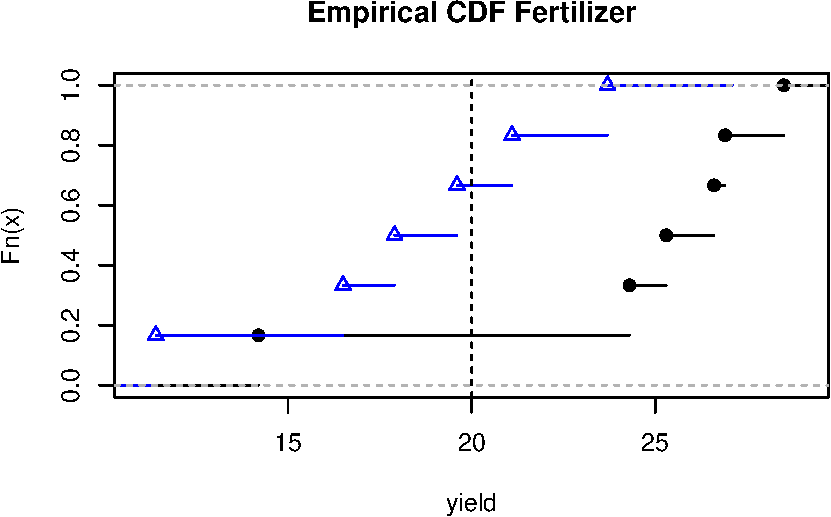
\includegraphics{class3slides-jan16_files/figure-beamer/unnamed-chunk-2-1.pdf}

\end{frame}

\begin{frame}{Empirical CDF}

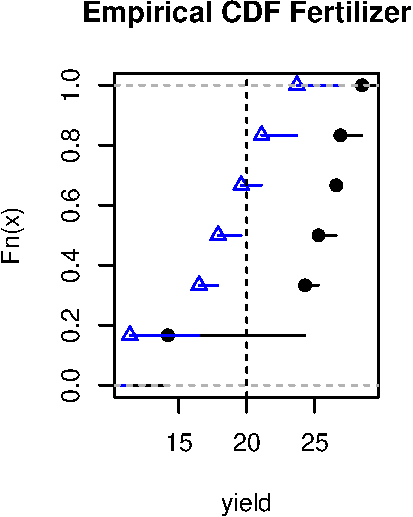
\includegraphics{class3slides-jan16_files/figure-beamer/unnamed-chunk-3-1.pdf}

\end{frame}

\begin{frame}{Summarizing a Distribution - Location}

Let \(x_1, x_2, \ldots, x_n\) be a sample from a distribution.

Sample mean: \[{\bar x}=\sum_{i=1}^{n}x_i/n\]

The \(p^{th}\) quantile of a distribution with CDF \(F\) is the value
\(x_p\) such that \({F}(x_p)=p\) or
\(x_p=F^{-1}(p)=\min\{x | F(x) \ge p \}\).

Sample percentile: A value \(\hat{x_{p}}\) such that:

\[\hat{x_{p}}= {\hat F}(p)^{-1}\]

For example, \(x_{0.25},x_{0.5},x_{0.75}\) are the \(25^{th},50^{th}\),
and \(75^{th}\) percentiles.

\end{frame}

\begin{frame}{Summarizing a Distribution - Scale}

Sample variance of \(x_1, x2, \ldots, x_n\) is

\[ s^2 =\frac{1}{n-1}\sum_{i=1}^{n}\left(x_i-{\bar x}\right)^2\]

The interquartile range is \(y_{0.75}-y_{0.25}\).

\end{frame}

\begin{frame}[fragile]{Summarizing Wheat Yield}

\begin{Shaded}
\begin{Highlighting}[]
\KeywordTok{summary}\NormalTok{(yA); }\KeywordTok{sd}\NormalTok{(yA);}\KeywordTok{quantile}\NormalTok{(yA,}\DataTypeTok{prob=}\KeywordTok{c}\NormalTok{(}\FloatTok{0.25}\NormalTok{,}\FloatTok{0.75}\NormalTok{))}
\end{Highlighting}
\end{Shaded}

\begin{verbatim}
##    Min. 1st Qu.  Median    Mean 3rd Qu.    Max. 
##   11.40   16.85   18.75   18.37   20.72   23.70
\end{verbatim}

\begin{verbatim}
## [1] 4.234934
\end{verbatim}

\begin{verbatim}
##    25%    75% 
## 16.850 20.725
\end{verbatim}

\begin{Shaded}
\begin{Highlighting}[]
\KeywordTok{summary}\NormalTok{(yB); }\KeywordTok{sd}\NormalTok{(yA); }\KeywordTok{quantile}\NormalTok{(yA,}\DataTypeTok{prob=}\KeywordTok{c}\NormalTok{(}\FloatTok{0.25}\NormalTok{,}\FloatTok{0.75}\NormalTok{))}
\end{Highlighting}
\end{Shaded}

\begin{verbatim}
##    Min. 1st Qu.  Median    Mean 3rd Qu.    Max. 
##   14.20   24.55   25.95   24.30   26.82   28.50
\end{verbatim}

\begin{verbatim}
## [1] 4.234934
\end{verbatim}

\begin{verbatim}
##    25%    75% 
## 16.850 20.725
\end{verbatim}

\end{frame}

\begin{frame}[fragile]{Results}

\begin{Shaded}
\begin{Highlighting}[]
\KeywordTok{mean}\NormalTok{(yA)-}\KeywordTok{mean}\NormalTok{(yB)}
\end{Highlighting}
\end{Shaded}

\begin{verbatim}
## [1] -5.933333
\end{verbatim}

\begin{itemize}
\tightlist
\item
  So there is a moderate/large difference in mean yield for these
  fertilizers.
\item
  Would you recommend B over A for future plantings?
\item
  Do you think these results generalize to a larger population?
\item
  Could the result be due to chance?
\end{itemize}

\end{frame}

\begin{frame}{Hypothesis Testing Via Randomization}

\begin{itemize}
\tightlist
\item
  Are the observed differences in yield due to fertilizer type?
\item
  Are the observed differences in yield due to plot-to-plot variation?
\end{itemize}

\end{frame}

\begin{frame}{Hypothesis Testing Via Randomization}

Hypothesis tests:

\begin{itemize}
\item
  \(H_0\) (null hypothesis): Fertilizer type does not affect yield.
\item
  \(H_1\) (alternative hypothesis): Fertilizer type does affect yield.
\item
  A statistical hypothesis evaluates the compatibility of \(H_0\) with
  the data
\end{itemize}

\end{frame}

\begin{frame}{Test Statistics and Null Distributions}

We can evaluate \(H_0\) by answering:

\begin{itemize}
\item
  Is a mean difference of -5.93 plausible/probable if H0 true?
\item
  Is a mean difference of -5.93 large compared to experimental noise?
\end{itemize}

\end{frame}

\begin{frame}{Test Statistics and Null Distributions}

\begin{itemize}
\item
  Compare \({\bar y}_a-{\bar y}_b\)=-5.93 (observed difference in the
  experiment) to values of \({\bar y}_a-{\bar y}_b\) that could have
  been observed if \(H_0\) were true.
\item
  Hypothetical values of \({\bar y}_a-{\bar y}_b\) that could have been
  observed under \(H_0\) are referred to as samples from the null
  distribution.
\end{itemize}

\end{frame}

\begin{frame}{Test Statistics and Null Distributions}

\begin{itemize}
\item
  \({\bar y}_a-{\bar y}_b\) is a function of the outcome of the
  experiment.
\item
  If a different experiment were performed then we would obtain a
  diffrent value of \({\bar y}_a-{\bar y}_b\).
\end{itemize}

\end{frame}

\begin{frame}{Test Statistics and Null Distributions}

\begin{itemize}
\tightlist
\item
  In this experiment we observed \({\bar y}_a-{\bar y}_b\)=-5.93.
\item
  If there was no difference between fertilizers then what other
  possible values of \({\bar y}_a-{\bar y}_b\) could have been observed?
\end{itemize}

\end{frame}

\begin{frame}{Experimental Procedure and Potential Outcomes}

The cards were shuffled and we were dealt B, R, B, R, \ldots{}

\begin{table}[]
\centering
\label{my-label}
\begin{tabular}{|l|l|l|l|l|l|}
\hline
B  & A  & B  & A  & B   & B  \\ \hline
B  & A  & A  & A  & B  & A  \\ \hline
\end{tabular}
\end{table}

Under this treatment assignment then the yields of the different plots
would be:

\begin{table}[]
\centering
\label{my-label}
\begin{tabular}{|l|l|l|l|l|l|}
\hline
B 26.9 & A 11.4 & B 26.6 & A 23.7 & B 25.3  & B 28.5 \\ \hline
B 14.2 & A 17.9 & A 16.5 & A 21.1 & B 24.3 & A 19.6 \\ \hline
\end{tabular}
\end{table}

\end{frame}

\begin{frame}{Experimental Procedure and Potential Outcomes}

Another potential treatment assignment under \(H_0\) is:

\begin{table}[]
\centering
\label{my-label}
\begin{tabular}{|l|l|l|l|l|l|}
\hline
B  & A  & B  & B  & A   & A  \\ \hline
A  & B  & B  & A  & A  & B  \\ \hline
\end{tabular}
\end{table}

The yields obtained under this assignment are:

\begin{table}[]
\centering
\label{my-label}
\begin{tabular}{|l|l|l|l|l|l|}
\hline
B 26.9 & A 11.4 & B 26.6 & B 23.7 & A 25.3  & A 28.5 \\ \hline
A 14.2 & B 17.9 & B 16.5 & A 21.1 & A 24.3 & B 19.6 \\ \hline
\end{tabular}
\end{table}

This data could occur of the experiment were run again.

\end{frame}

\begin{frame}[fragile]{Experimental Procedure and Potential Outcomes}

\begin{itemize}
\tightlist
\item
  Under this hypothetical assignment the mean difference is:
\end{itemize}

\begin{Shaded}
\begin{Highlighting}[]
\NormalTok{yA <-}\StringTok{ }\KeywordTok{c}\NormalTok{(}\FloatTok{11.4}\NormalTok{,}\FloatTok{25.3}\NormalTok{,}\FloatTok{28.5}\NormalTok{,}\FloatTok{14.2}\NormalTok{,}\FloatTok{21.1}\NormalTok{,}\FloatTok{24.3}\NormalTok{)}
\NormalTok{yB <-}\StringTok{ }\KeywordTok{c}\NormalTok{(}\FloatTok{26.9}\NormalTok{,}\FloatTok{26.6}\NormalTok{,}\FloatTok{23.7}\NormalTok{,}\FloatTok{17.9}\NormalTok{,}\FloatTok{16.5}\NormalTok{,}\FloatTok{19.6}\NormalTok{)}
\KeywordTok{mean}\NormalTok{(yA-yB)}
\end{Highlighting}
\end{Shaded}

\begin{verbatim}
## [1] -1.066667
\end{verbatim}

This represents an outcome of the experiment in a universe where:

\begin{enumerate}
\def\labelenumi{\arabic{enumi}.}
\item
  The treatment assignment is B, A, B, B, A, A, A, B, B, A, A, B
\item
  \(H_0\) is true (i.e., \(\mu_A=\mu_B\), where \(\mu_A,\mu_B\) are the
  mean yields of fertilizers A and B).
\end{enumerate}

\end{frame}

\begin{frame}{The Null distribution}

\begin{itemize}
\tightlist
\item
  What potential outcomes would we see if \(H_0\) is true?
\item
  Compute \({\bar y}_a-{\bar y}_b\) for each possible treatment
  assignment.
\end{itemize}

\end{frame}

\begin{frame}{The Null Distribution}

\begin{itemize}
\tightlist
\item
  For each treatment assignment compute
  \[\delta_i={\bar y}_a-{\bar y}_b, i=1,2,\ldots,924.\]
\item
  \(\left\{\delta_1, \delta_2, \ldots, \delta_{924}\right\}\) enumerates
  all pre-randomisation outcomes assuming no treatment effect.
\item
  Since each treatment assignment is equally likely under the null
  distribution, a probability distribution of experimental results if
  \(H_0\) is true can be described as
\end{itemize}

\[{\hat F}(y)=\frac{\#(\delta_i \le y)}{924}.\] This is called the
randomisation distribution.

\end{frame}

\begin{frame}{Randomization Distribution}

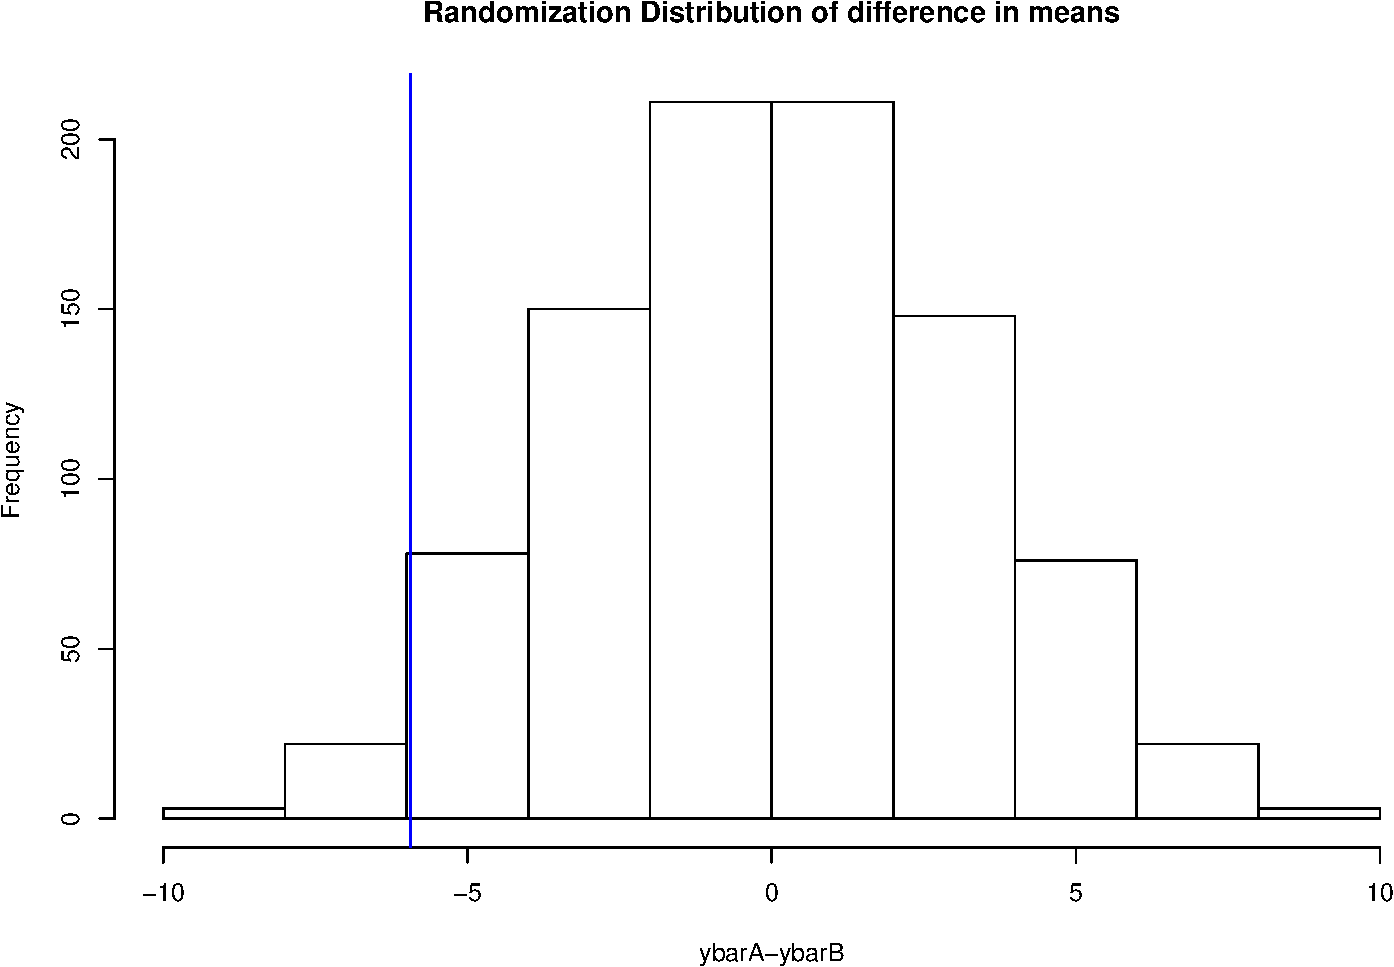
\includegraphics{class3slides-jan16_files/figure-beamer/unnamed-chunk-7-1.pdf}

\end{frame}

\begin{frame}{Hypothesis Testing}

\begin{itemize}
\tightlist
\item
  Is there any contradiction between \(H_0\) and the observed data?
\item
  Calculate
\end{itemize}

\[{\hat F}(-5.93)=\frac{\#(\delta_i \le -5.93)}{924}.\]

\end{frame}

\begin{frame}{Hypothesis Testing}

\begin{itemize}
\tightlist
\item
  A P-value is the probability, under the null hypothesis of obtaining a
  more extreme than the observed result.
\end{itemize}

\[ \text{P-value}=P\left(\delta \le -5.93 \right)\]

\begin{itemize}
\item
  A small P-value implies evidence \textbf{against} null hypothesis.
\item
  If the P-value is large does this imply that the null is true?
\end{itemize}

\end{frame}

\begin{frame}{Randomization Test}

\begin{itemize}
\item
  Assume \(H_0\) is true.
\item
  Calculate the difference in means for every possible way to split the
  data into two samples of size 6.
\item
  This would result in \({{12}\choose{6}}=924\) differences.
\item
  Calculate the probability of observing a value as extreme of more
  extreme than the observed value of the test statistic
  (\emph{P-value}).
\item
  If the P-value is small then there are two possible explanations:
\end{itemize}

\begin{enumerate}
\def\labelenumi{\arabic{enumi}.}
\item
  An unlikely value of the statistic has occurred, or
\item
  The assumption that \(H_0\) is true is incorrect.
\end{enumerate}

\begin{itemize}
\tightlist
\item
  If the P-value is large then the hypothesis test is inconclusive.
\end{itemize}

\end{frame}

\end{document}
